\documentclass[10pt]{article}
\usepackage[margin=0.82in]{geometry}
\usepackage{amsmath,amssymb,amsthm,booktabs,graphicx,microtype,float,placeins}
\usepackage[font=small,skip=3pt]{caption}
\usepackage[hidelinks]{hyperref}
\setlength{\parindent}{0pt}
\setlength{\parskip}{3pt plus 1pt minus 1pt}
\setlength{\textfloatsep}{7pt plus 2pt minus 2pt}
\setlength{\intextsep}{7pt plus 2pt minus 2pt}
\newtheorem{theorem}{Theorem}
\newtheorem{proposition}[theorem]{Proposition}
\newtheorem{corollary}[theorem]{Corollary}
\theoremstyle{definition}
\newtheorem{definition}[theorem]{Definition}
\title{\vspace{-1.7em}\textbf{Creativity as Constrained Rarity}\par
\vspace{-2pt}\large Semantics, Compression, and Representation in Finite Program Spaces\vspace{-0.5em}}
\author{J. R. Landers}
\date{\vspace{-1.4em}}

\begin{document}
\maketitle
\vspace{-1.5em}

\begin{abstract}
We develop a representation-conditional theory of constrained rarity and test
it in two finite program spaces.  A semantic fiber collects all programs of a
fixed size that compute the same function; compression locates the first
nonempty fiber and rarity measures its mass under an explicit prior.  General
results formalize semantics-preserving padding, the prior-dependence of rarity,
and the loss of distinctions under semantic coarsening.  Sorting supplies
independent decision-tree and adjacent-swap theorems as well as an exhaustive
enumeration of 221,832 correct four-input comparator networks.  Boolean
synthesis supplies an exact root-decomposition recurrence and all 256
three-input functions in NAND, NOR, and AND/OR/NOT formula languages.
Syntax-free semantic descriptors predict minimum formula size after complete
descriptor-class holdout with $R^2=0.613$--$0.656$, beyond 1,000 matched nulls
in each language ($p<0.001$).  Yet NAND--NOR rank correlations are only 0.548
for minimum size, 0.376 for boundary surprisal, and 0.264 for canonical
compression gain.  Likewise, 12 optimal sorting networks share one entropy
curve but have 12 distinct full output-distribution trajectories.  Semantic
structure constrains difficulty, while numerical rarity, compression, and
geometric rigidity remain conditional on language, prior, and resolution.
\end{abstract}

\section{Finite semantic fibers}

Let a finite graded representation language be
$E_{\mathcal L}=\bigsqcup_{\ell\ge0}E_{\mathcal L,\ell}$, with size
$|e|=\ell$ for $e\in E_{\mathcal L,\ell}$.  A semantic evaluation map
\[
 \operatorname{eval}_{\mathcal L}:E_{\mathcal L}\longrightarrow F
 \tag{1}
\]
sends syntax to a task or function in $F$.

\begin{definition}[Fiber, boundary, and surprisal]
For $f\in F$, define
\[
 A_{\mathcal L,\ell}(f)
 =\{e\in E_{\mathcal L,\ell}:\operatorname{eval}_{\mathcal L}(e)=f\},
 \qquad
 L_{\mathcal L}^*(f)=\min\{\ell:A_{\mathcal L,\ell}(f)\ne\varnothing\}.
 \tag{2}
\]
Under the uniform prior conditional on exact size, the boundary probability
and surprisal are
\[
 q_{\mathcal L}(f)
 =\frac{|A_{\mathcal L,L^*}(f)|}{|E_{\mathcal L,L^*}|},
 \qquad
 R_{\mathcal L}(f)=-\log_2q_{\mathcal L}(f).
 \tag{3}
\]
For a frozen compiler or reference construction of length
$L_{0,\mathcal L}(f)$, compression gain is
$G_{\mathcal L}(f)=L_{0,\mathcal L}(f)-L_{\mathcal L}^*(f)$.
\end{definition}

The operational creativity profile is retained as a vector
\[
 \mathcal C_{\mathcal L}(f)
 =\bigl(S(f),G_{\mathcal L}(f),R_{\mathcal L}(f),\psi(f)\bigr),
 \tag{4}
\]
where $S$ records semantic correctness and $\psi$ records semantic structure.
The notation deliberately exposes the representation language.  Multiplying
the components can enforce conjunction, but it does not make their units or
priors intrinsic.

\subsection{Why redundant correct programs proliferate}

\begin{theorem}[Injective semantic padding]
Suppose there are $m$ maps
$T_j:E_{\mathcal L,\ell}\to E_{\mathcal L,\ell+\delta}$ such that each $T_j$
is injective, their images are pairwise disjoint, and
$\operatorname{eval}(T_j(e))=\operatorname{eval}(e)$.  Then for every $f$,
\[
 |A_{\mathcal L,\ell+\delta}(f)|\ge
 m|A_{\mathcal L,\ell}(f)|.
 \tag{5}
\]
If the same maps can be iterated with the same properties, then
$|A_{\mathcal L,\ell+k\delta}(f)|\ge m^k|A_{\mathcal L,\ell}(f)|$.
\end{theorem}

\begin{proof}
For fixed $j$, semantic preservation maps the fiber at $\ell$ into the fiber
at $\ell+\delta$.  Injectivity preserves its cardinality; disjoint images let
the $m$ cardinalities add.  Iteration gives the second claim by induction.
\end{proof}

For a sorted comparator-network output, appending any of the six comparators
preserves correctness.  Thus $m=6$ and $\delta=1$.  For ordered AND/OR/NOT
formulas, choose a variable $x_i$ and one of
\[
 e\land(x_i\lor\neg x_i),\qquad e\lor(x_i\land\neg x_i).
 \tag{6}
\]
Across three variables these give six disjoint syntactic contexts with
$m=6$ and $\delta=3$.  The same theorem therefore captures redundant volume
in both experimental universes without claiming that their grammars are
identical.

\subsection{Why rarity requires a declared prior}

\begin{theorem}[Prior relativity]
Let $E$ and $F$ be finite and let $\operatorname{eval}:E\to F$ be surjective.
For every strictly positive probability mass function $q$ on $F$, there is a
prior $P$ on $E$ whose induced semantic distribution is exactly $q$.
\end{theorem}

\begin{proof}
For each $f$, choose any conditional distribution $w_f$ supported on the
nonempty fiber $\operatorname{eval}^{-1}(f)$ and set
$P(e)=q(f)w_f(e)$ when $\operatorname{eval}(e)=f$.  Then
$\sum_{e:\operatorname{eval}(e)=f}P(e)=q(f)$, and summing over $f$ gives total
mass one.
\end{proof}

Thus semantic probability can be reassigned arbitrarily unless the program
language and prior are fixed.  Cross-language stability is empirical evidence
for a semantic component; it cannot turn rarity itself into an invariant.

\subsection{Why semantic resolution matters}

\begin{proposition}[Coarsening cannot reveal distinctions]
Let $\phi:X\to Y$ be a fine semantic representation and $c:Y\to Z$ a
coarsening.  The partition of $X$ induced by $c\circ\phi$ is coarser than the
partition induced by $\phi$.  In particular,
\[
 |(c\circ\phi)(X)|\le |\phi(X)|.
 \tag{7}
\]
Equality at the coarse level does not imply equality at the fine level.
\end{proposition}

\begin{proof}
If $\phi(x)=\phi(x')$, then applying $c$ gives
$c(\phi(x))=c(\phi(x'))$.  Hence every fine equivalence class lies inside a
coarse class, proving the inequality and the final non-implication.
\end{proof}

\section{Sorting: bounds, paths, and exact networks}

\subsection{Comparison trees}

For $n$ distinct keys, each input has one of $n!$ order types.  A deterministic
comparison algorithm induces a binary decision tree whose reached leaf must
identify the correct output order.

\begin{theorem}[Comparison boundary and random-label thinness]
Every correct comparison decision tree has at least $n!$ reached leaves and
worst-case depth
\[
 d\ge\lceil\log_2(n!)\rceil.
 \tag{8}
\]
Fix a tree shape and any distribution over its internal comparison labels.  If
each leaf output is labeled independently and uniformly from $S_n$, then
\[
 \Pr(\text{correct on every order type})
 \le \left(\frac1{n!}\right)^{n!}.
 \tag{9}
\]
\end{theorem}

\begin{proof}
Two distinct order types cannot reach the same leaf in a correct tree, since
that leaf has one output label.  Therefore at least $n!$ leaves are reached,
while a depth-$d$ binary tree has at most $2^d$ leaves, proving (8).

Condition on all internal comparison labels, which fixes the routing.  If two
order types collide, correctness has conditional probability zero.  Otherwise
the $n!$ order types reach distinct leaves.  Their independent uniform labels
simultaneously match the $n!$ required outputs with probability
$(1/n!)^{n!}$.  Averaging over the internal labels proves (9).
\end{proof}

The depth bound is necessary, not a claim that every depth at the information
bound is attainable by legal comparisons.  The probability bound describes
the declared uninformed leaf-label prior, not human algorithm design.

\subsection{Adjacent-swap paths}

Let $G_n$ be the Cayley graph of $S_n$ generated by adjacent transpositions
$s_1,\ldots,s_{n-1}$.  Write $I=\operatorname{inv}(\sigma)$ and let
$\Gamma_L(\sigma)$ be the exact-length-$L$ paths from $\sigma$ to the identity.

\begin{theorem}[Geodesic length, parity, and redundant paths]
The graph distance from $\sigma$ to the identity is $I$.  Moreover,
$\Gamma_L(\sigma)=\varnothing$ unless $L\ge I$ and $L-I$ is even.  For every
$m\ge0$,
\[
 |\Gamma_{I+2m}(\sigma)|
 \ge (n-1)^m|\Gamma_I(\sigma)|,
 \qquad
 \frac{|\Gamma_I(\sigma)|}{|\Gamma_{I+2m}(\sigma)|}
 \le(n-1)^{-m}.
 \tag{10}
\]
\end{theorem}

\begin{proof}
An adjacent swap changes inversion number by exactly one.  Reaching inversion
zero therefore takes at least $I$ steps, and repeatedly swapping an adjacent
inversion gives a path of length $I$.  The parity of inversion number flips at
every step, so an endpoint-correct path must satisfy $L-I$ even.

Take any geodesic word of length $I$.  After it reaches the identity, append
$m$ pairs $(s_{i_1},s_{i_1}),\ldots,(s_{i_m},s_{i_m})$.  Each pair is the
identity, so the endpoint is unchanged.  There are $(n-1)^m$ choices, and the
resulting words are distinct because their first $I$ symbols recover the
geodesic and their final pairs recover the choices.  Applying this construction
to every geodesic proves (10).
\end{proof}

\subsection{Four-input comparator networks}

The experiment uses oblivious comparator sequences over the six unordered
wire pairs, not adaptive decision trees or adjacent-swap words.  Each sequence
is checked on all 24 inputs.  No sequence through length four sorts; exactly
12 of $6^5=7{,}776$ length-five sequences sort.  Hence
\[
 q_5(\mathrm{sort})=0.00154321,
 \qquad R_5=9.340\ \text{bits}.
 \tag{11}
\]
Correct counts rise to 900, 16,800, and 204,120 at lengths six, seven, and
eight.  The padding theorem guarantees only 72, 432, and 2,592 descendants of
the 12 optima at those lengths; the larger exact counts include genuinely
different longer routes.  The fraction that reaches the sorted state before
its final comparison is 8.0\%, 32.1\%, and 49.4\%.

\begin{figure}[!htbp]
  \centering
  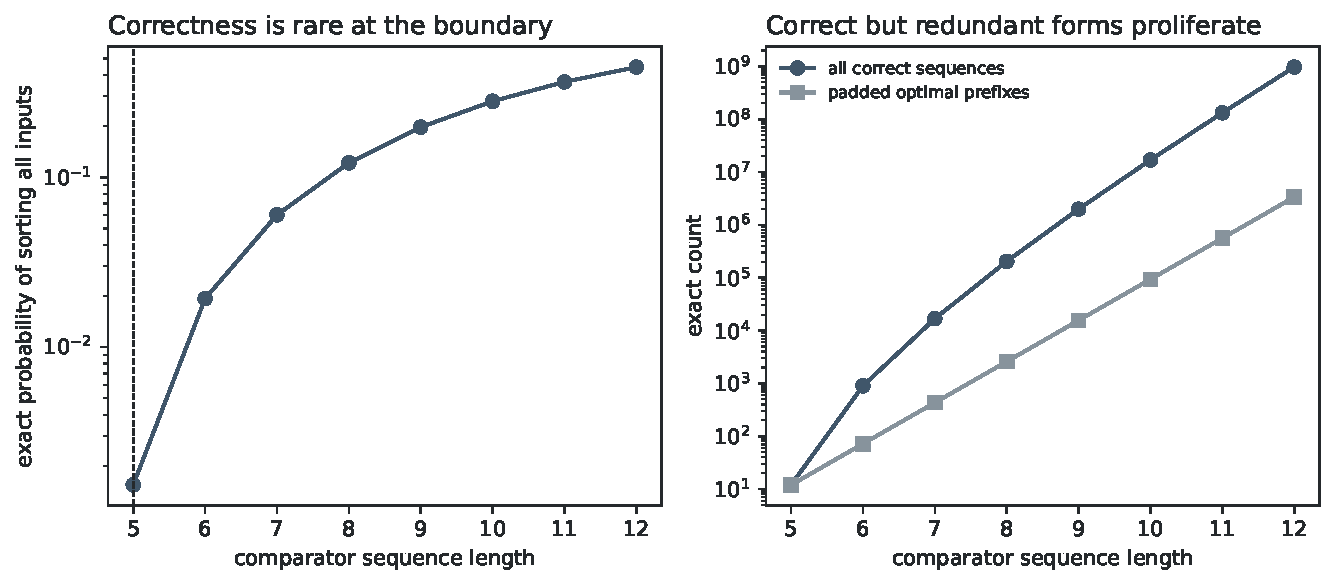
\includegraphics[width=0.88\textwidth]{../../experiments/creativity-sorting-networks/figures/sorting_creativity.pdf}
  \caption{Exact four-input sorting counts.  Correctness is rare at the
  five-comparator boundary (left).  Correct sequences then proliferate much
  faster than the guaranteed family obtained by padding optimal prefixes
  (right).  The prior is uniform over the six comparators conditional on exact
  sequence length.}
  \label{fig:sorting-counts}
\end{figure}
\FloatBarrier

\section{Boolean formulas: exact semantic synthesis}

Let a formula be an ordered rooted tree with leaves $x_0,x_1,x_2$ and internal
nodes from a fixed gate basis.  Size is the number of gates.  Truth tables are
eight-bit semantic values.

\begin{theorem}[Exact root-decomposition recurrence]
Let $C_\ell(t)$ be the number of ordered formulas of size $\ell$ with truth
table $t$.  If $\mathcal O_r$ is the set of $r$-ary gates, then
\[
 C_0(t)=|\{i:\operatorname{eval}(x_i)=t\}|,
 \tag{12}
\]
and for $\ell\ge1$,
\[
 C_\ell(t)=
 \sum_{r\ge1}\ \sum_{o\in\mathcal O_r}\
 \sum_{\ell_1+\cdots+\ell_r=\ell-1}\
 \sum_{o(t_1,\ldots,t_r)=t}
 \prod_{j=1}^r C_{\ell_j}(t_j).
 \tag{13}
\]
Consequently this dynamic program counts every formula exactly once.
\end{theorem}

\begin{proof}
Every non-leaf formula has a unique root gate $o$, an ordered tuple of unique
root subformulas, and a unique ordered composition
$\ell_1+\cdots+\ell_r=\ell-1$ of their gate counts.  Conversely, every choice
enumerated on the right constructs one formula of size $\ell$ and semantic
value $t$.  The two constructions are inverse.
\end{proof}

For NAND or NOR, summing (13) over truth tables yields
\[
 |E_\ell|=\operatorname{Catalan}(\ell)3^{\ell+1}.
 \tag{14}
\]
For AND/OR/NOT, with $T_0=3$,
\[
 T_\ell=T_{\ell-1}+2\sum_{i=0}^{\ell-1}T_iT_{\ell-1-i}.
 \tag{15}
\]
Both identities are independently checked at every enumerated size.

\begin{proposition}[Input-renaming invariance]
If the grammar treats all variables symmetrically, then for every input
permutation $\pi$ and every $\ell$, relabeling leaves is a size-preserving
bijection
\[
 A_{\mathcal L,\ell}(f)\longleftrightarrow
 A_{\mathcal L,\ell}(f\circ\pi).
 \tag{16}
\]
Thus minimum size, exact fiber count, and boundary surprisal are constant on
input-permutation orbits.
\end{proposition}

\begin{proof}
Replace every leaf $x_i$ by $x_{\pi(i)}$.  This operation preserves the tree
and gate count, changes its semantics by input relabeling, and is inverted by
$\pi^{-1}$.
\end{proof}

The recurrence synthesizes all 256 functions.  The unique hardest function in
the NAND language is three-bit parity at 14 gates.  Exactly 373,248 of
38,375,290,837,080 size-14 formulas compute it, giving 26.615 bits of boundary
surprisal.  Across all functions, minimum NAND size and boundary surprisal have
Spearman $\rho=0.948$, whereas canonical-compiler compression gain and
surprisal have $\rho=-0.037$.  Difficulty and rarity align strongly at the
boundary; compiler-relative compression is a separate quantity.

\begin{figure}[!htbp]
  \centering
  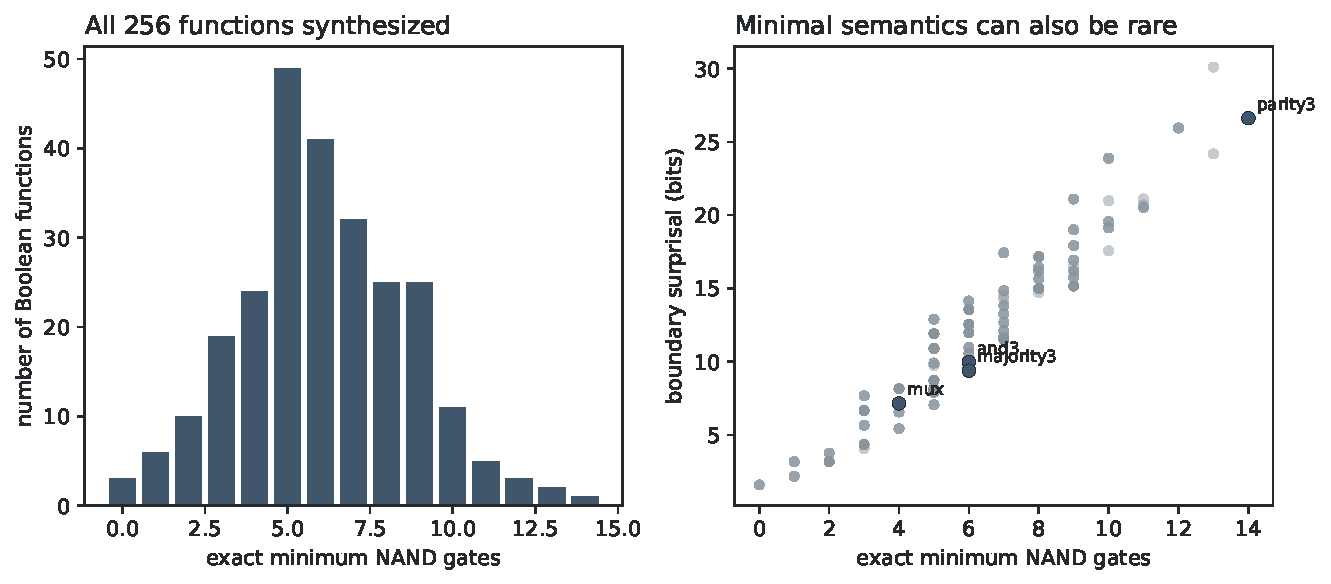
\includegraphics[width=0.88\textwidth]{../../experiments/creativity-boolean-synthesis/figures/boolean_synthesis_creativity.pdf}
  \caption{Exact NAND synthesis.  All 256 functions are reached by size 14
  (left).  Boundary surprisal rises with minimum size but retains meaningful
  within-size variation (right); labeled functions are fixed before analysis.}
  \label{fig:boolean-synthesis}
\end{figure}
\FloatBarrier

\section{Semantic prediction and representation stability}

For each Boolean function, the syntax-free descriptor $\psi(f)$ contains
signed output bias, sorted variable influences, Walsh--Fourier energy at
degrees zero through three, algebraic degree, and the size of the
input-permutation stabilizer.  These give 36 exact descriptor classes.  The
same semantic coordinates are used for all three languages in
Figure~\ref{fig:boolean-atlas}.

\begin{figure}[!htbp]
  \centering
  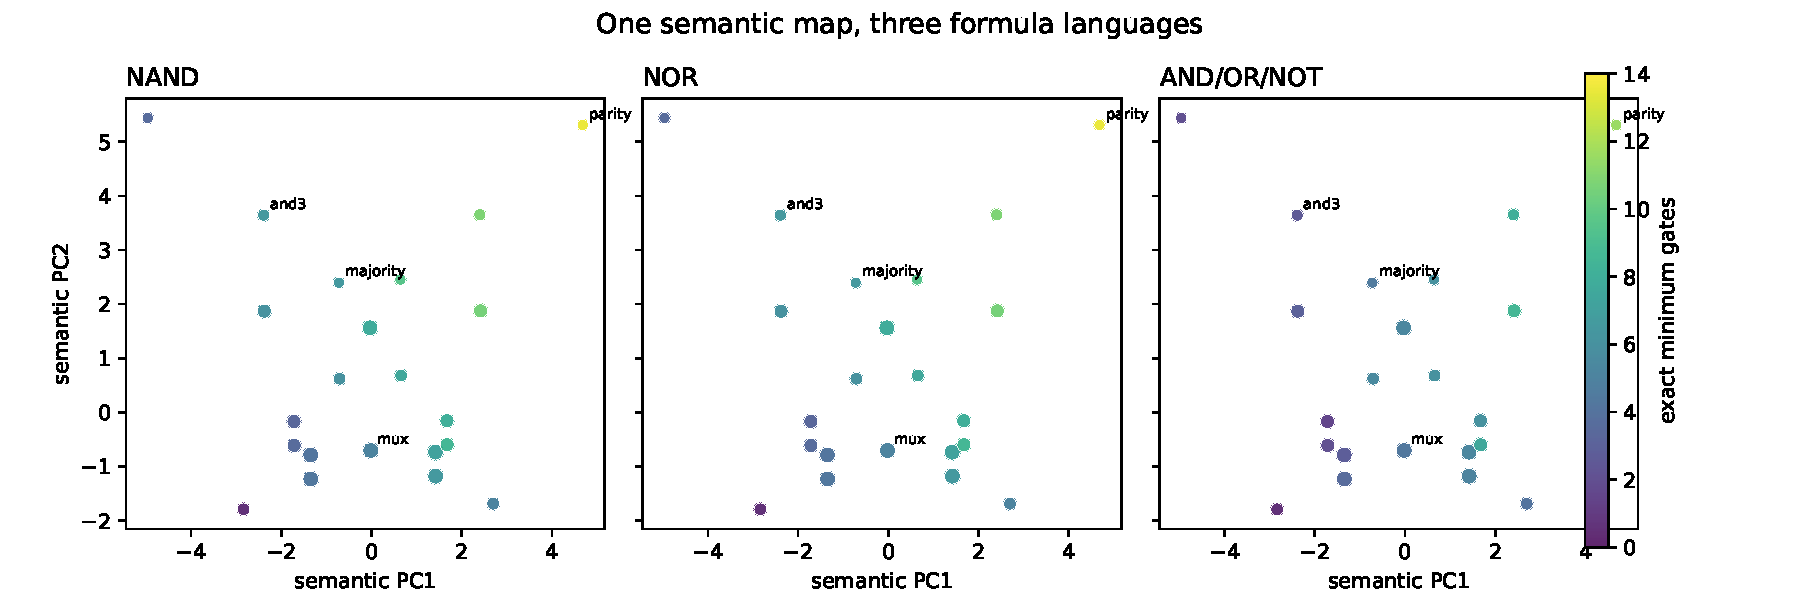
\includegraphics[width=0.96\textwidth]{../../experiments/creativity-boolean-atlas/figures/boolean_semantic_atlas.pdf}
  \caption{A common syntax-free semantic map colored by exact minimum size.
  Point area records projected multiplicity.  Persistent color structure
  reflects semantic constraint; color changes across panels expose
  representation dependence.  Statistical tests use the full descriptor,
  not the two-dimensional projection.}
  \label{fig:boolean-atlas}
\end{figure}
\FloatBarrier

\subsection{Cross-language stability}

\begin{table}[!htbp]
\centering
\small
\begin{tabular}{lrrr}
\toprule
Language pair & Minimum size & Boundary surprisal & Compression gain \\
\midrule
NAND / NOR & 0.548 & 0.376 & 0.264 \\
NAND / AND--OR--NOT & 0.805 & 0.739 & 0.612 \\
NOR / AND--OR--NOT & 0.805 & 0.739 & 0.601 \\
\bottomrule
\end{tabular}
\caption{Spearman correlations across all 256 functions.  Minimum complexity
has a substantial semantic component, while rarity and canonical compression
are more sensitive to the primitive language.}
\label{tab:stability}
\end{table}

The NAND--NOR comparison holds the truth-table function fixed.  De Morgan
duality can map a function to a different dual function, but that does not make
the cost of the original semantic target representation-independent.

\subsection{Group-held-out prediction and matched nulls}

A seven-nearest-neighbor predictor is evaluated under three protocols:
leave one function out; remove its full input-permutation orbit (80 orbits);
and remove its complete invariant descriptor class (36 classes).  The last
protocol removes all feature-identical twins.

\begin{table}[!htbp]
\centering
\small
\begin{tabular}{lrrrr}
\toprule
Language & Function held out & Orbit held out & Descriptor held out & Strict RMSE \\
\midrule
NAND & 0.831 & 0.726 & 0.613 & 1.583 \\
NOR & 0.833 & 0.729 & 0.643 & 1.522 \\
AND--OR--NOT & 0.920 & 0.859 & 0.656 & 1.161 \\
\bottomrule
\end{tabular}
\caption{Held-out $R^2$ for exact minimum gate count.  The strict protocol
removes the near-duplicate leakage present in ordinary leave-one-out
prediction; a majority of variance remains predictable.}
\label{tab:prediction}
\end{table}

The null test permutes minimum sizes within exact strata of signed bias,
algebraic degree, and stabilizer size, preserving those coarse explanations.
Across 1,000 repetitions the null mean and central 95\% interval are $-0.064$
$[-0.271,0.118]$ for NAND, $-0.068$ $[-0.269,0.106]$ for NOR, and $0.014$
$[-0.149,0.155]$ for AND/OR/NOT.  No replicate reaches the corresponding
observed strict $R^2$, so the finite-simulation $p$-value is $1/1001<0.001$ in
each language.

\begin{figure}[!htbp]
  \centering
  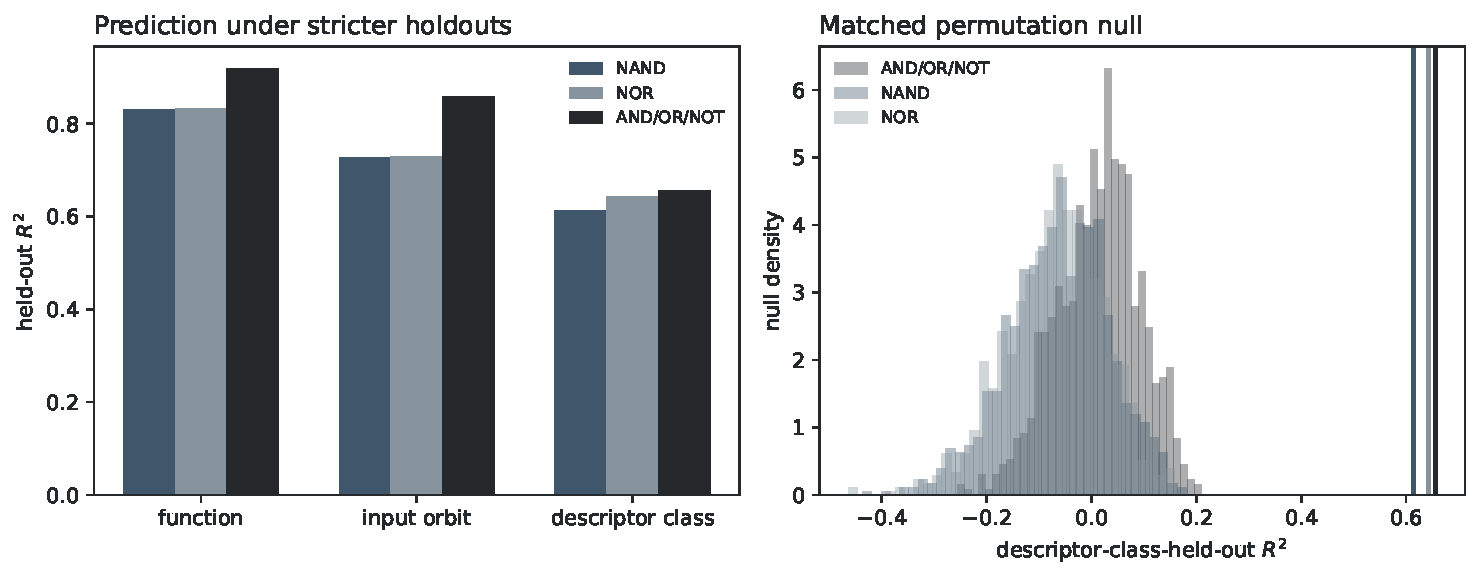
\includegraphics[width=0.94\textwidth]{../../experiments/creativity-atlas-validation/figures/boolean_validation.pdf}
  \caption{Boolean validation.  Prediction attenuates under progressively
  stricter semantic holdouts (left) but remains far beyond matched null
  distributions (right).  Vertical lines are the observed descriptor-class
  results.}
  \label{fig:boolean-validation}
\end{figure}
\FloatBarrier

\section{Sorting trajectories at two semantic resolutions}

For comparator prefix $e_{1:t}$, let $Y_t$ be its output on a uniformly
sampled input permutation and
\[
 p_t(y)=\Pr(Y_t=y),\qquad
 H_t=-\sum_y p_t(y)\log_2p_t(y).
 \tag{17}
\]
The entropy trajectory $(H_0,\ldots,H_L)$ is a coarsening of the full path
$(p_0,\ldots,p_L)$.  A single global wire permutation acts on all 24
coordinates at every step; the full trajectory is represented by the
lexicographically least member of this 24-element orbit.

\begin{table}[!htbp]
\centering
\small
\begin{tabular}{rrrrr}
\toprule
Length & Correct words & Entropy paths & Full paths / wires & Raw full paths \\
\midrule
5 & 12 & 1 & 12 & 12 \\
6 & 900 & 27 & 756 & 756 \\
7 & 16,800 & 147 & 4,356 & 4,356 \\
8 & 204,120 & 497 & 15,036 & 15,036 \\
\bottomrule
\end{tabular}
\caption{Exact semantic-trajectory counts.  Several comparator words can
induce one full path, and many full paths can induce one entropy curve.  The
fixed ascending target anchors wire order, so the declared global wire quotient
does not merge additional correct paths.}
\label{tab:sorting}
\end{table}

All 12 optimal networks share one entropy curve but have 12 distinct full
paths.  This is the coarsening proposition in action: equality after coarsening cannot be
read backward as equality of computation.  Absolute full-path diversity then
grows to 756, 4,356, and 15,036.

\begin{figure}[!htbp]
  \centering
  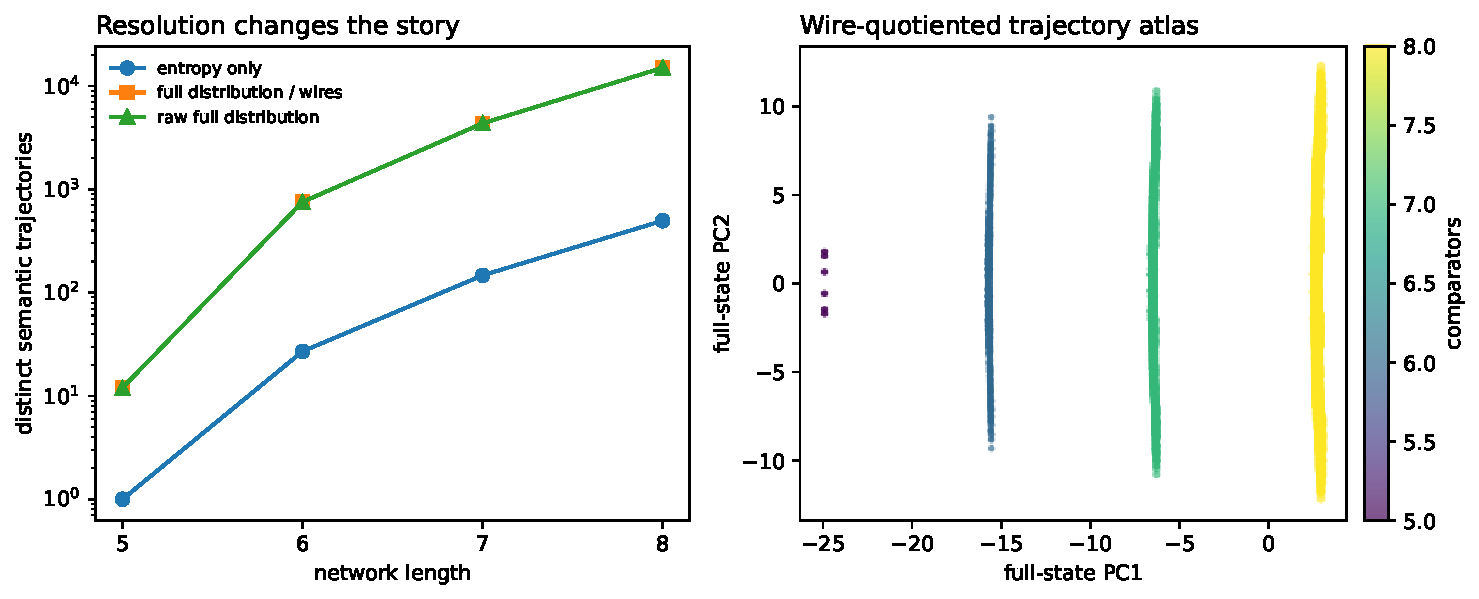
\includegraphics[width=0.94\textwidth]{../../experiments/creativity-atlas-validation/figures/sorting_validation.pdf}
  \caption{Resolution test.  Entropy merges orders of magnitude more paths
  than the full output distribution (left).  The descriptive PCA of canonical
  full trajectories (right) shows within-length variation; separated length
  bands partly reflect interpolation to a common time grid, so inference uses
  exact counts rather than projected coordinates.}
  \label{fig:sorting-validation}
\end{figure}
\FloatBarrier

\section{Interpretation}

The mathematical and numerical results support five claims.
\begin{enumerate}
  \setlength{\itemsep}{0pt}
  \setlength{\parskip}{0pt}
  \setlength{\parsep}{0pt}
  \item Correct programs form semantic fibers, and compression identifies the
  first nonempty fiber.
  \item Semantics-preserving padding produces large families of redundant
  correct representations, but exact growth depends on the grammar.
  \item Semantic structure predicts synthesis difficulty beyond input-renaming
  twins and coarse matched null properties.
  \item Rarity and baseline-relative compression are not properties of a
  semantic function alone; their values require a language and prior.
  \item Apparent geometric rigidity can be created by a coarse statistic.
\end{enumerate}

Thus constrained rarity is neither pure subjectivism nor a universal
coordinate.  A defensible claim has the form
\[
 \text{successful compression inside a semantically constrained space}
 \quad\text{relative to }(\mathcal L,P,L_0,\psi).
 \tag{18}
\]
The framework does not establish human originality, aesthetic value, discovery
effort, or representation-independent Kolmogorov complexity.  It makes the
dependencies of an operational claim explicit and falsifiable.

For formal mathematics, the immediate lesson is methodological.  Isolation in
one Lean embedding is not evidence of profundity.  A stronger analysis should
compare theorem statements with proof journeys at several semantic
resolutions, remove complete equivalence neighborhoods rather than individual
declarations, and demand stability under vocabulary ablation, repository
matching, and alternative formal encodings.  The finite experiments show that
a semantic signal can survive hard controls; they also show why one
representation can overstate it.

\paragraph{Reproducibility.}
The repository contains every script, frozen configuration, artifact, and
figure used here.  Counts are checked against independent recurrences or
brute-force enumeration, null draws use seed 0, and all five experiments and
the document build run locally without cloud services or model APIs.

\end{document}
